\documentclass[../main]{subfiles}
\ifSubfilesClassLoaded{
    \dominitoc
    \tableofcontentsfile
    \pagenumbering{arabic}
    \setcounter{page}{1}
	\setcounter{chapter}{2}
}{}
\begin{document}
\chapter{Convergence de la relaxation}
\graphicspath{{./},{07-Relaxation/}}
\minitoc

Le processus de relaxation que nous proposons dans l'algorithme CxSOM est une méthode originale pour construire des connexions bidirectionnelles entre cartes. Deux cartes connectées de cette façon jouent alors un rôle symétrique. La relaxation est en même temps une recherche d'un ensemble de Best Matching units par consensus.
Dans cette section, nous apportons un formalisme et des éléments d'étude de la méthode de relaxation proposée dans cette thèse et étudierons expérimentalement la relaxation sur un exemple.

\section{Du calcul cellulaire au calcul à l'échelle d'une carte}

L'algorithme de relaxation proposé dans le modèle CxSOM s'appuie sur le modèle de relaxation développé sur ds architectures de cartes auto-organisatrices cellulaires, dans lesquelles les calculs sont réalisés à l'échelle du neurone \cite{khouzam_neural_2014}.

\section{Formalisme de l'algorithme de relaxation}

La recherche du BMU par consensus dans l'architecture CxSOM peut se traduire par une recherche de maximum dans l'architecture, donc un problème d'optimisation.
La relaxation proposée est une heuristique de cette recherche de maximum.
Nous n'avons pas résolu analytiquement le problème d'optimisation. Nous formulons cependant le problème dans cette section.

\subsection{Problème d'optimisation}

La relaxation constitue une maximisation de l'activité globale de chaque carte de l'architecture.
Nous cherchons donc un ensemble de valeurs que nous notons $\mathbf{\bmu} = (\bmu\m{1}, \cdots, \bmu\m{n})$.
Ecrivons ici les équations à l'équilibre, c'est à  dire dans le cas où un BMU est défini dans chaque carte.
%ecrire pb de maximisation.
A l'issue de la relaxation, dans chaque carte $i$, l'activité globale est définie par~:

\begin{equation}
	a_g\m{i}(p\m{i},\bmu\m{i_0}, \cdots, \bmu\m{i_K}) = \sqrt{a_e\m{i}(p\m{i},\inpx\m{i})(\frac{1}{2}a_e\m{i}(p\m{i},\inpx\m{i}) + \frac{1}{2}a_c\m{i}(p\m{i},\bmu\m{i_0}, \cdots, \bmu\m{i_K})}
\end{equation}

Rappelons que l'activité contextuelle $a_c$ est définie comme la moyenne des activités sur chaque couche de poids contextuels~:
\begin{equation}
	a_c(p\m{i}, \bmu\m{i_0}, \cdots, \bmu\m{i_K}) = \frac{1}{k+1}\sum_{k=0}^{K}{a_{ck}(p\m{i}, \bmu\m{i_k})}
\end{equation}

Enfin, le BMU d'une carte est défini comme la position où l'activité globale d'une carte est maximale. Donc, à l'équilibre, le BMU est l'ensemble des positions $(\bmu\m{1}, \cdots, \bmu\m{n})$ satisfaisant les équations ; 
\begin{equation}
	\forall i, \: \bmu\m{i} = \argmax_{p\m{i}}(a_g\m{i}(p\m{i},\bmu\m{i_0}, \cdots \bmu\m{i_K}))
\end{equation}

Autrement dit, chaque valeur $\bmu\m{i}$ maximise $a_g\m{i}(\bmu\m{i},\inpx_m{i},\bmu\m{i_1}, \cdots, \bmu\m{i_K})$. 
$a_g\m{i}$ étant à valeurs positives pour tout $i$, le consensus s'exprime de façon équivalente comme une solution du problème d'optimisation multi-objectif suivant~:

\begin{equation}\label{eq:opti}
	\begin{cases}
	\text{Maximiser}\;& \sum_{i = 1}^n a_g\m{i}((\bmu\m{i},\inpx_m{i},\bmu\m{i_1}, \cdots, \bmu\m{i_K})) \\
	\text{Sous Contrainte }\; &\forall i, \; \bmu\m{i} = \argmax_{p\m{i}}a_g\m{i}(p\m{i},\bmu\m{i_0}, \cdots \bmu\m{i_K})
	\end{cases}
\end{equation}

En fonction des poids des cartes, il n'est pas assuré qu'une solution existe ni qu'elle soit unique. Au contraire, dans un cas quelconque, ce genre de problème qui s'apparente à la recherche d'un optimum de Pareto n'a pas de solution, il s'agit de trouver un compromis.
Ici, l'objectif dépend de la disposition des poids des cartes. Nous cherchons à étudier l'existence d'une solution dans le cadre particulier des poids de cartes auto-organisatrices.

\subsection{Heuristique de recherche~: relaxation}

La relaxation définie dans le modèle est une heuristique de recherche du maximum par déplacements dans l'espace des positions $(\bmu\m{1},\codts, \bmu\m{n})$.

Notons $(\mathbf{\bmu})_\tau = (\bmu\m{0}_\tau,\cdots,\bmu\m{n}_\tau)$ la suite définie par l'évolution des BMUs des $N$ cartes d'une architecture lors de la relaxation.
La suite $(\mathbf{\bmu})_\tau$ est une suite définie par récurrence par $\mathbf{\bmu}_{\tau+1} = \mathbf{f}(\mathbf{\bmu}_\tau)$ avec $\mathbf{f} = (f\m{0},\cdots,f\m{n}) : [0,1]^N \rightarrow [0,1]^N$. $\mathbf{f}$ ne dépend pas de $\tau$. 

Détaillons l'évolution de cette suite.
Pour clarifier les notations, définissons pour chaque carte~$i$ $\hat{p}\m{i}_\tau$, comme la position maximisant l'activité globale de la carte $i$ à l'instant $\tau$.

\begin{equation}
\begin{gathered}
\hat{p}\m{i}_{\tau} = \argmax_{p\m{i}}(a_g\m{i}(p\m{i},\bmu\m{i_0}_\tau, \cdots \bmu\m{i_K}_\tau))\\
 i_0, \cdots i_K \: \text{indices des cartes nourrissant la carte $i$}.
\end{gathered}
\label{eq:pstar}
\end{equation}

$a_g\m{i}$ est une fonction des poids de la carte $\w\ext\m{i}, \w\cont\m{i}$ et de son entrée externe $\inpx\m{i}$. Lors du processus de relaxation, les poids et l'entrée $\inpx\m{i}$ restent fixes. Le calcul de $a_g$ ne dépend pas de $\tau$. Pour toute carte $i$, $\hat{p}\m{i}_{\tau}$ dépend donc uniquement de $(\bmu\m{i_0}_\tau, \cdots \bmu\m{i_K}_\tau)$ et l'équation d'évolution s'écrit alors: 
\begin{equation}
\bmu\m{i}_{\tau+1} = 
\begin{cases}
\bmu\m{i}_{\tau} + sgn(\hat{p}\m{i}_{\tau} - \bmu\m{i}_{\tau}) \times \delta \; & \text{si $\hat{p}\m{i}_{\tau} - \bmu\m{i}_{\tau} > \delta$ } \\
\hat{p}\m{i}_{\tau} \; \text{sinon}	
\end{cases}
\label{eq:evolution}
\end{equation}

En posant $f\m{i}$ la partie droite de l'équation \ref{eq:evolution}, on peut donc écrire: 
\begin{equation}
\bmu\m{i}_{\tau +1} = f\m{i}(\bmu\m{0}_\tau,\cdots,\bmu\m{n}_\tau)
\label{eq:fonction}
\end{equation}

Soit, pour l'ensemble des composantes: 
\begin{equation}
\mathbf{\bmu}_{\tau+1} = \mathbf{f}(\mathbf{\bmu}_\tau)
\end{equation}

La relaxation se traduit ainsi par une recherche de point fixe de la suite $(\mathbf{\bmu})_{\tau}$, soit une position $\mathbf{\bmu}$ telle que:
\begin{equation}
\mathbf{\bmu} = \mathbf{f}(\mathbf{\bmu})
\label{eq:suite}
\end{equation}

Un point fixe de la fonction $f$ est bien une solution du système d'équations~\ref{eq:opti}.
Si $f$ admet un point fixe, alors ce point fixe est aussi un point fixe pour la suite $(\mathbf{\bmu})_\tau$. Cependant, rien ne garantit que ce point fixe existe, ni que la suite converge.

L'évolution de la suite $(\mathbf{\bmu})_{\tau}$ dépend de son initialisation.
Lors de l'apprentissage du modèle, nous prenons comme état initial $(\bmu\m{0}_0, \cdots , \bmu\m{n}_0)$ : 
\begin{equation}
\begin{cases}
\bmu\m{0}_0 = \argmax_{p\m{0}} a_e(p\m{0},\inpx\m{0})\\
\cdots \\
\bmu\m{n}_0 = \argmax_{p\m{n}} a_e(p\m{n},\inpx\m{n})\\
\end{cases}
\label{eq:init}
\end{equation}
Nous étudierons dans ce chapitre la relaxation pour $(\bmu\m{0}_0, \cdots , \bmu\m{n}_0)$ quelconques.

\subsection{Relaxation et notion de \emph{Best Matching Unit}}

La notion de Best Matching Unit est définie au sein de l'algorithme d'apprentissage d'une carte de Kohonen, comme l'unité possédant l'activité maximale pour une entrée fixée. 
Cette activité dépend de l'entrée présentée et des poids de la carte, mais peut aussi dépendre d'autres variables pour d'autres modèles de carte, tels que l'état de la carte au temps précédent pour les cartes récurrentes, ou dans notre cas les positions des BMU des cartes adjacentes.
Dans le modèle classique de carte auto-organisatrice, le BMU possède les propriétés suivantes~:
\begin{itemize}
	\item La BMU est seulement relative à l'état de la carte (activités) et sa ou ses entrées. Notons qu'en règle générale, ce BMU est unique. Cependant, plusieurs poids peuvent être égaux dans une carte et correspondre à l'activité maximale. Le nombre de n\oe{}uds étant fini, l'égalité de plusieurs poids d'une carte suite à l'évolution de l'algorithme est de probabilité nulle.
	\item La recherche du BMU est déterministe
\end{itemize}

La relaxation est une méthode de recherche dynamique du BMU. Pour les propriétés du BMU ci dessus soient respectées, il est nécessaire que~: 
\begin{itemize}
	\item La recherche du BMU converge. S'il n'existe pas de point de convergence, nous ne pouvons pas définir un BMU unique pour la carte. 
	\item La solution est unique~: la valeur trouvée à l'issue de la relaxation, à savoir le point de convergence s'il existe, ne dépend pas des conditions initiales de la relaxation. Le BMU est alors relatif à seulement l'état des poids de la carte et non des conditions initiales.
\end{itemize}

Nous chercherons à évaluer si ces deux conditions sont remplies lors de la relaxation.
Notons que dans l'algorithme CxSOM, les BMUs sont initialisés à la position du maximum de l'activité externe dans chaque carte. 
Nous effectuerons l'analyse de la relaxation pour des conditions initiales quelconques, mais il est important de noter que ce choix d'initialisation permettra d'éviter certains cas de non-convergence.

Nous montrerons expérimentalement qu'il n'existe pas toujours un unique point fixe, notamment lorsque les poids sont répartis aléatoirement au début de l'apprentissage, ce qui entraîne alors une non-convergence de la relaxation. 
Cependant, nous observons que ces cas de non-convergence n'influencent pas le dépliement ultérieur des cartes, ce qui est permis par l'initialisation des positions au maximum de l'entrée externe.
Nous observera expérimentalement qu'à la fin de l'apprentissage, la disposition des poids permet l'existence d'un unique point fixe qui est indépendant de l'initialisation des valeurs de $\bmu\m {i}_{\tau}$.

Ce chapitre présente des points d'analyse empirique de ce processus de relaxation, réalisée sur des cartes prenant des dispositions d'entrées particulières: un cercle en deux et trois dimensions.
La démarche expérimentale est la suivante:
Nous évaluerons d'abord le taux de convergence de la relaxation dans les expériences citées ci-dessus.
Nous proposons ensuite une visualisation de l'unicité du point fixe en fonction des conditions initiales de la relaxation. Enfin, nous étudierons comment le choix du pas de relaxation $\Delta$ influence la relaxation.

\section{Etude expérimentale de la convergence de la relaxation}

Nous nous intéressons ici  à un processus d'apprentissage complet d'une architectures de deux cartes. Les entrés $\inpx\m{1}$ et $\inpx\m{2}$ présentées sont les coordonnées de points situés sur un cercle de centre 0.5 et de rayon 0.5. Nous détaillerons le choix de disposition d'entrées par la suite~; notons simplement que ces entrées sont normalisées, chaque prenant toutes les valeurs entre 0 et 1.
Pendant l'apprentissage, nous effectuons des phases de test régulières à poids figés, sur 5000 points tirés selon les mêmes distributions d'entrées. Nous avons compté, pour chaque entrée, le nomre de pas nécessaires à la convergence de la relaxation. En pratique, l'algorithme de relaxation s'arrête si la relaxation dépasse $\tau_{max}= 1000$ itérations~; nous considérerons donc que la relaxation n'a pas atteint un point de convergence si le nombre de pas de relaxation a atteint ces $\tau_{max}$ itérations lors de l'expérience. \'A partir de ces valeurs, nous pouvons traçer le nombre de pas moyen nécessaire à la convergence (en prenant en compte les cas dans lesquel la relaxation ne converge pas), ainsi que le taux de convergence~: la proportion d'entrées sur les 5000 entrées tests pour lesquelles la relaxation a convergé.
Nous répétons 10 fois l'apprentissage complet et les tests, sur le même espace d'entrée mais des éléments différents ainsi que des cartes initialisées aléatoirement.
Nous traçons ainsi en figure~\ref{fig:conv_evolution} la moyenne et l'écart type du nombre moyen de pas de relaxation et du taux de convergence obtenues sur ces 10 répétitions.

Plusieurs situations peuvent se traduire par une non-convergence de la relaxation:
\begin{itemize}
\item La relaxation évolue vers un point de convergence, mais trop lentement pour y arriver en moins de 1000 itérations
\item La relaxation évolue vers un cycle limite composé d'un nombre limité d'unités étant alternativement Best Matching Units
\item La relaxation évolue sans répétition de motifs dans les cartes, il s'agit d'une évolution chaotique.
\end{itemize}

Le premier cas est évité car la limite de 1000 itérations est assez grande par rapport à la taille de la carte, les cartes étant de taille 500 et le pas d'évolution de la relaxation d'une dizaine d'unités. 
La convergence, si elle existe, est donc rapide. Les cas de non-convergence concernent alors la deuxième et la troisième situation.
Nous observerons plus précisément les trajectoires dans la section suivante; on s'intéresse ici seulement à la question de la convergence.

La figure\ref{fig:conv_evolution} montre qu'au début de l'apprentissage, lorsque les poids sont initialisés aléatoirement, la relaxation atteint rarement un point de convergence. Lorsque les cartes sont dépliée, la relaxation évolue vers un point de convergence dans plus de $90 \%$ des cas. Cette évolution est similaire pour des architecture de deux et trois cartes.

Nous en  concluons que la convergence de la relaxation dépend complètement de la disposition des poids. Elle converge dans plus de 90 \% des cas lorsque les poids sont bien dépliés, mais seulement dans 20\% des cas au début de l'apprentissage lorsque les poids ne présentent aucune forme de continuité et d'organisation.
Le fait que la relaxation ne converge pas en début d'apprentissage ne perturbe cependant pas le dépliement des poids.

\begin{figure}
\centering
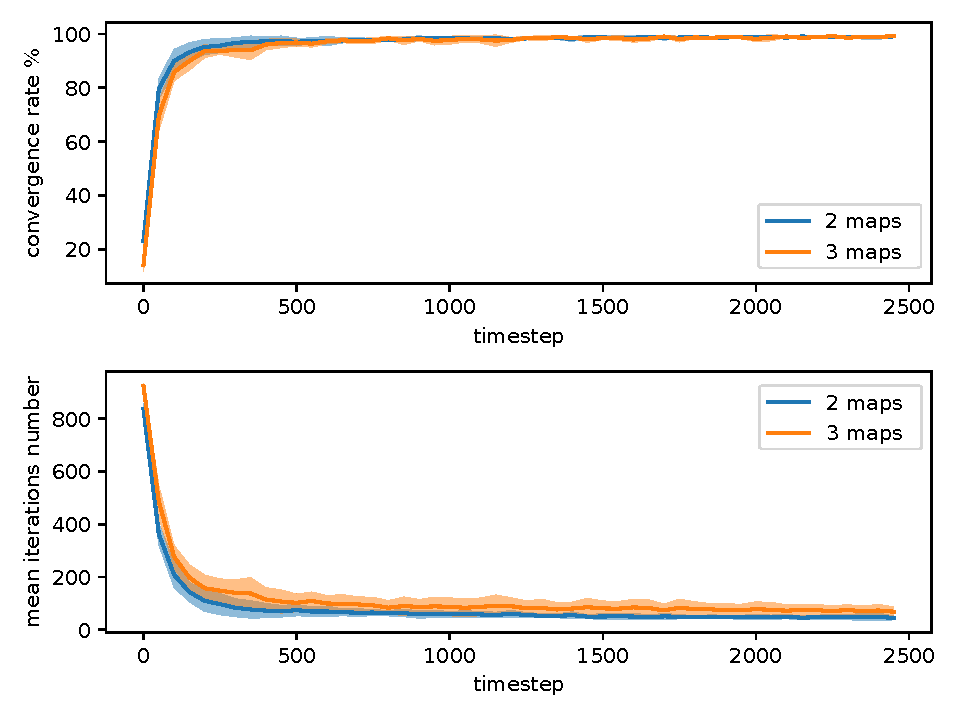
\includegraphics[width=0.7\textwidth]{1D_conv_evolution_total.pdf}
\caption{En haut: évolution de la moyenne et l'écart-type du taux de convergence lors de la relaxation au cours de l'apprentissage sur deux et trois cartes 1D. En bas: évolution du nombre moyen de pas nécessaires à la convergence de la relaxation.
Chaque point est calculé sur un échantillon de 1000 relaxations au temps t, évaluées sur des entrées différentes prises aléatoirement sur le cercle. La moyenne et l'écart-type sont réalisés sur 10 apprentissages séparés.}
\label{fig:conv_evolution}
\end{figure}

\section{Analyse paramétrique de la relaxation}

% Nous avons montré que la relaxation converge dans 90\% des cas dans l'expérience lorsque les poids des cartes sont dépliés à la fin de l'apprentissage. 
% Dans ce cas, les poids externes sont ordonnés de façon monotone entre $0$ et $1$ et les poids contextuels présentent une continuité locale et plusieurs minima et maxima au long de la carte.

\subsection{Trajectoires de relaxation\label{sec:pf}}

Nous étudions dans cette partie l'évolution de plusieurs processus de relaxation lancés sur les mêmes poids de cartes, a présent pour pour une seule entrée externe fixée, mais avec des valeurs d'initialisation de relaxation $\mathbf{\bmu}_0$ différents.

Pour un problème à deux cartes, il est possible de rechercher de façon exhaustive une solution de l'équation \ref{eq:opti}, qui s'écrit alors : 
\begin{equation}
	\begin{cases}
		\bmu\m{1} = \argmax_p a_g\m{1}(p, \bmu\m{2})
		\bmu\m{2} = \argmax_q a_g\m{2}(q, \bmu\m{2})
	\end{cases}
\end{equation}

En figure \ref{fig:diff_relax_t1_notraj} et \ref{fig:diff_relax_notraj}, nous représentons en carte de coloration les quantités $\lvert \hat{p}\m{1} - p\m{1} \rvert$ et $\lvert \hat{p}\m{2} - p\m{2}\rvert$ en fonction de $p\m{1},p\m{2} \in [0,1]$, pour la configuration des poids au début et celle à la fin de l'apprentissage.
Le point fixe s'il existe, est alors à une position $p\m{1},p\m{2}$ vérifiant :
\begin{equation*}
\begin{cases}
\hat{p}\m{1} = p\m{1}\\
\hat{p}\m{2} = p\m{2}\\
\end{cases}
\end{equation*}
Ces positions sont représentées par les zones en violet sur chaque graphique.
Pour $t = 0$ (figure~\ref{fig:diff_relax_t1_notraj}, nous remarquons un couple de position $p\m{1}, p\m{2}$, en $(0.1, 0.75)$, dans lequels les deux valeurs sont nulles. Ce couple semble être un hasard de l'exemple.
A la fin de l'apprentissage( figure~\ref{fig:diff_relax_notraj}) une structure apparaît dans les valeurs des différences, et un point où les deux différences sont nulles existe à l'intersection des deux zones en violet.

La relaxation est un déplacement de la valeur $\bmu\m{1}_\tau, \bmu\m{2}_\tau)$ dans l'espace des positions $p\m{1}, p\m{2}$. 
Pour la même entrée et les mêmes poids, nous lançons 200 trajectoires de relaxation, initialisées à des valeurs $\bmu\m{1}_0,\bmu\m{2}_0$ différents, choisies aléatoirement sur les cartes.
Les valeurs obtenues à l'issue de chaque relaxation sont représentées par les point noir sur les figures \ref{fig:diff_relax_t1_notraj} et \ref{fig:diff_relax_notraj}.

La figure\ref{fig:diff_relax_t1_notraj} nous montre qu'au début de l'apprentissage, la fonction de relaxation évolue vers plusieurs points en fonction des conditions initiales, représentés par les points noirs distincts. 
Ces points d'attraction représentent différent types d'évolution de la suite. Les trajectoires évoluant vers $(0.1, 0.75)$ évoluent vers un point fixe. Nous observons également un attracteur en cycle limite.
Afin de mieux représenter les trajectoires, ous traçons en \ref{fig:champ_0} représente le champ des déplacement à effectuer de $(\bmu\m{1}_\tau,\bmu\m{2}_\tau)$ lors de la relaxation en fonction de la position courante. 
Nous y traçons les trajectoires aboutissants aux points présentés en figure \ref{fig:diff_relax_t1_notraj}.
Ces champs de déplacement permettent d'observer les comportements de point fixe et cycles limite des attracteurs.

Nous pouvons ensuite comparer ces deux figures à celles obtenues en fin d'apprentissage, représentées en figure \ref{fig:diff_relax_notraj} et \ref{fig:champ_9999}.
Sur ces tracés, nous observons un seul point d'attraction pour les 200 trajectoires. La relaxation ne dépend donc plus des conditions initiales.
Ce point correspond à la position où les deux différences $\lvert \hat{p}\m{1} - p\m{1} \rvert$ et $\lvert \hat{p}\m{2} - p\m{2}\rvert$ sont nulles.
La figure \ref{fig:champ_9999} présente le champ de déplacement des BMUs en fonction de la position courante. Les trajectoires suivent les zones où l'une ou l'autre des différences est nulle, pour mener à la position stable. 
En réalisant ces tests sur plusieurs exemples, nous avons remarqué ce  même schéma en fin d'apprentissage pour les différences $\lvert \hat{p}\m{i} - p\m{i} \rvert$.

Cette propriété vient de la disposition ordonnée des poids externes à la fin de l'apprentissage et de la formule du calcul d'activité.
\'A la fin de l'apprentissage, $a_e(\inpx,p)$ présente un seul maximum. 
De plus, l'activité globale correspond à la modulation de l'activité contextuelle par les valeurs de l'activité externe. Donc, à $\inpx\m{1}$ fixé ,$\hat{p}\m{1} = \argmax_p\m{1} a_g(p\m{1}, p\m{2})$ reste dans une zone restreinte lorsque $p\m{2}$ varie (de même pour $a_g\m{2}$). 
La relaxation évoluera donc vers cette zone réduite.
Cette propriété est illustrée en figure\ref{fig:w006}.
Nous y faisons figurer les poids des deux cartes et les valeurs de $\hat{p}\m{1}$ et $\hat{p}\m{2}$ obtenues en faisant varier $p\m{1}, p\m{2}$ dans tout l'espace des positions possibles.

D'après cet exemple, nous formulons l'hypothèse que le dépliement ordonné des poids externes dans une carte en 1D est une condition suffisante à l'existence d'un unique point fixe. 
Dans ce cas, la relaxation permet de trouver ce point fixe.


\begin{figure}
\begin{minipage}{0.5\textwidth}
\centering
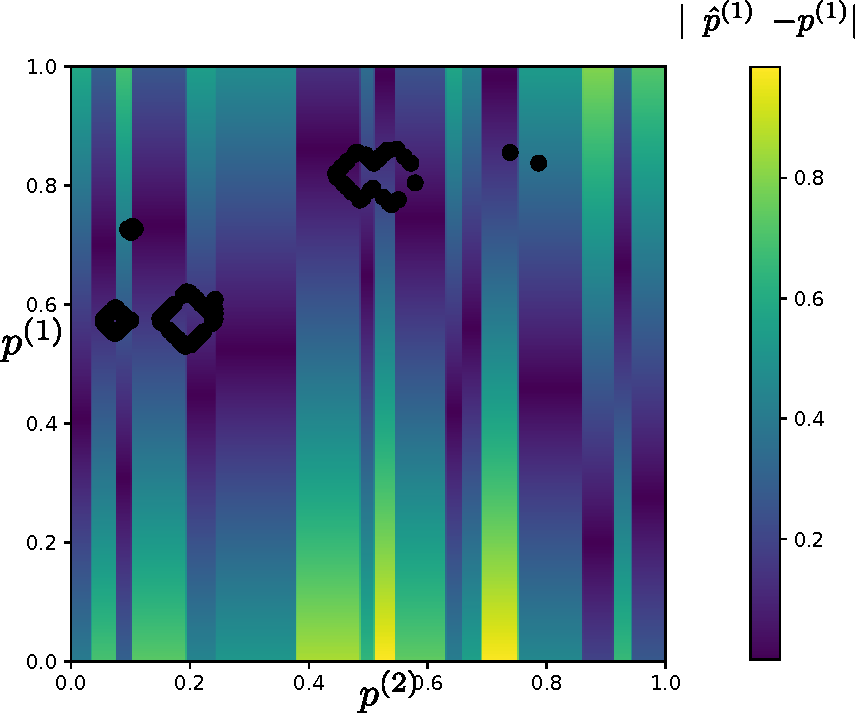
\includegraphics[width=\textwidth]{champ_X_006_t1_notraj.pdf}
\end{minipage}
\begin{minipage}{0.5\textwidth}
\centering
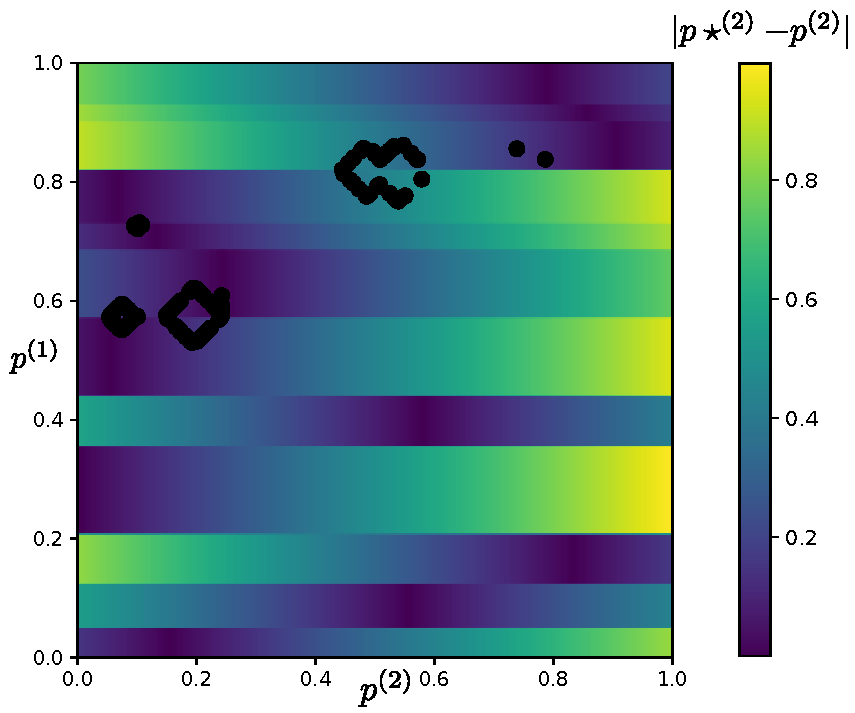
\includegraphics[width=\textwidth]{champ_Y_006_t1_notraj.pdf}
\end{minipage}
\caption{Valeur de ${\hat{p}}\m{1} - p\m{1}$, resp. ${\hat{p}}\m{2} - p\m{2}$ à $t=0$ ,lorsque les poids sont encore aléatoiremement disposés dans chaque carte.
 ${\hat{p}}\m{1}$ ne dépend que de $p\m{2}$ : on peut donc tracer cette valeur selon deux dimensions pour chaque carte. Les zones où cette valeur est nulle sont en violet sur le graphique. Les points fixes, s'il existent, sont aux positions de différence nulle pour $M\m{1}$ et $M\m{2}$. Les points noirs représentent les points de convergence pour 200 trajectoires de relaxation, lancées pour différents $\bmu_0\m{1}, \bmu_0\m{2}$.}
 
\label{fig:diff_relax_t1_notraj}
\end{figure}

\begin{figure}
\begin{minipage}{0.5\textwidth}
\centering
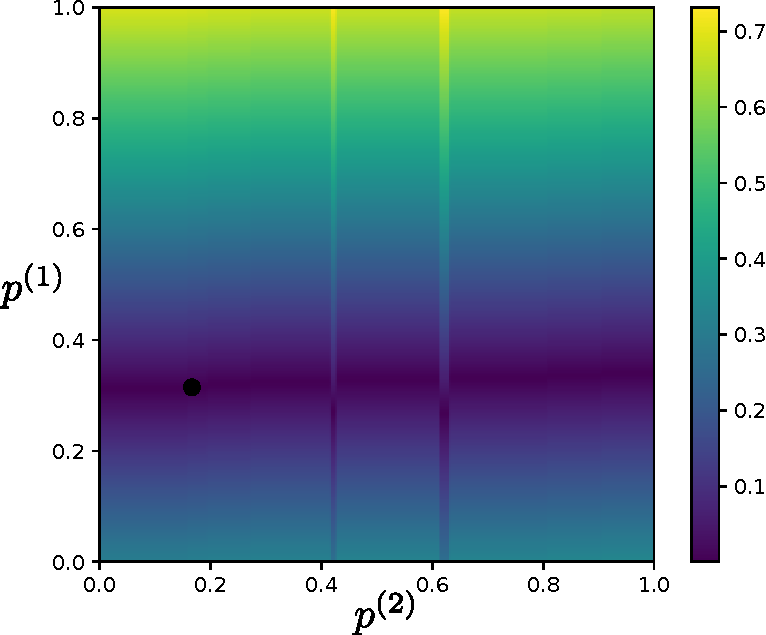
\includegraphics[width=\textwidth]{champ_X_006_notraj.pdf}
\end{minipage}
\begin{minipage}{0.5\textwidth}
\centering
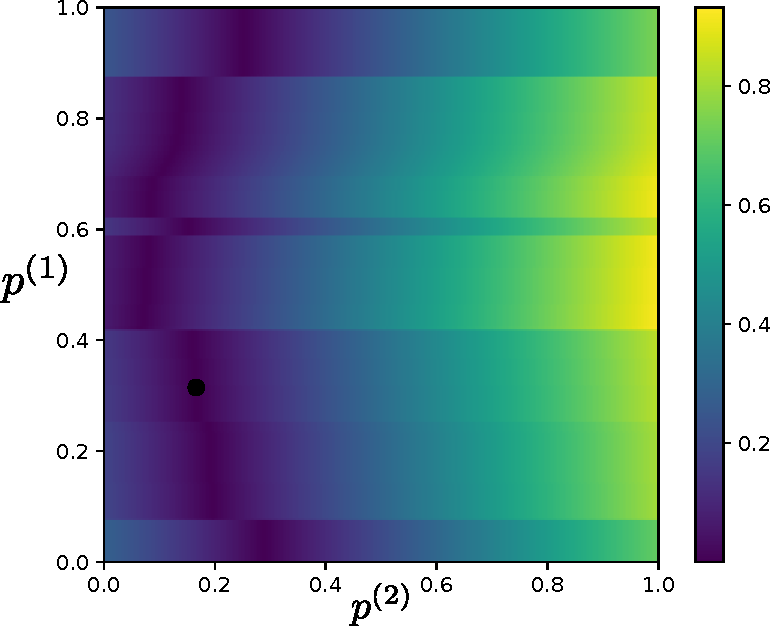
\includegraphics[width=\textwidth]{champ_Y_006_notraj.pdf}
\end{minipage}
\caption{Valeur de ${\hat{p}}\m{1} - p\m{1}$, resp. ${\hat{p}}\m{2} - p\m{2}$, lorsque les cartes sont organisées telles qu'en figure \ref{fig:w006}. ${\hat{p}}\m{1}$ ne dépend que de $p\m{2}$ : on peut donc tracer cette valeur selon deux dimensions pour chaque carte. Les zones où cette valeur est nulle sont en violet sur le graphique. Les points fixes, s'il existent, sont aux positions de différence nulle pour $M\m{1}$ et $M\m{2}$. Les points noirs représentent les points d'arrivée de la relaxation pour 50 trajectoires de relaxation, lancées pour différents $\bmu_0\m{1}, \bmu_0\m{2}$. La relaxation semble présenter un point de convergence, qui se situe sur un point fixe de la fonction de relaxation.}
\label{fig:diff_relax_notraj}
\end{figure}

\begin{figure}
\centering
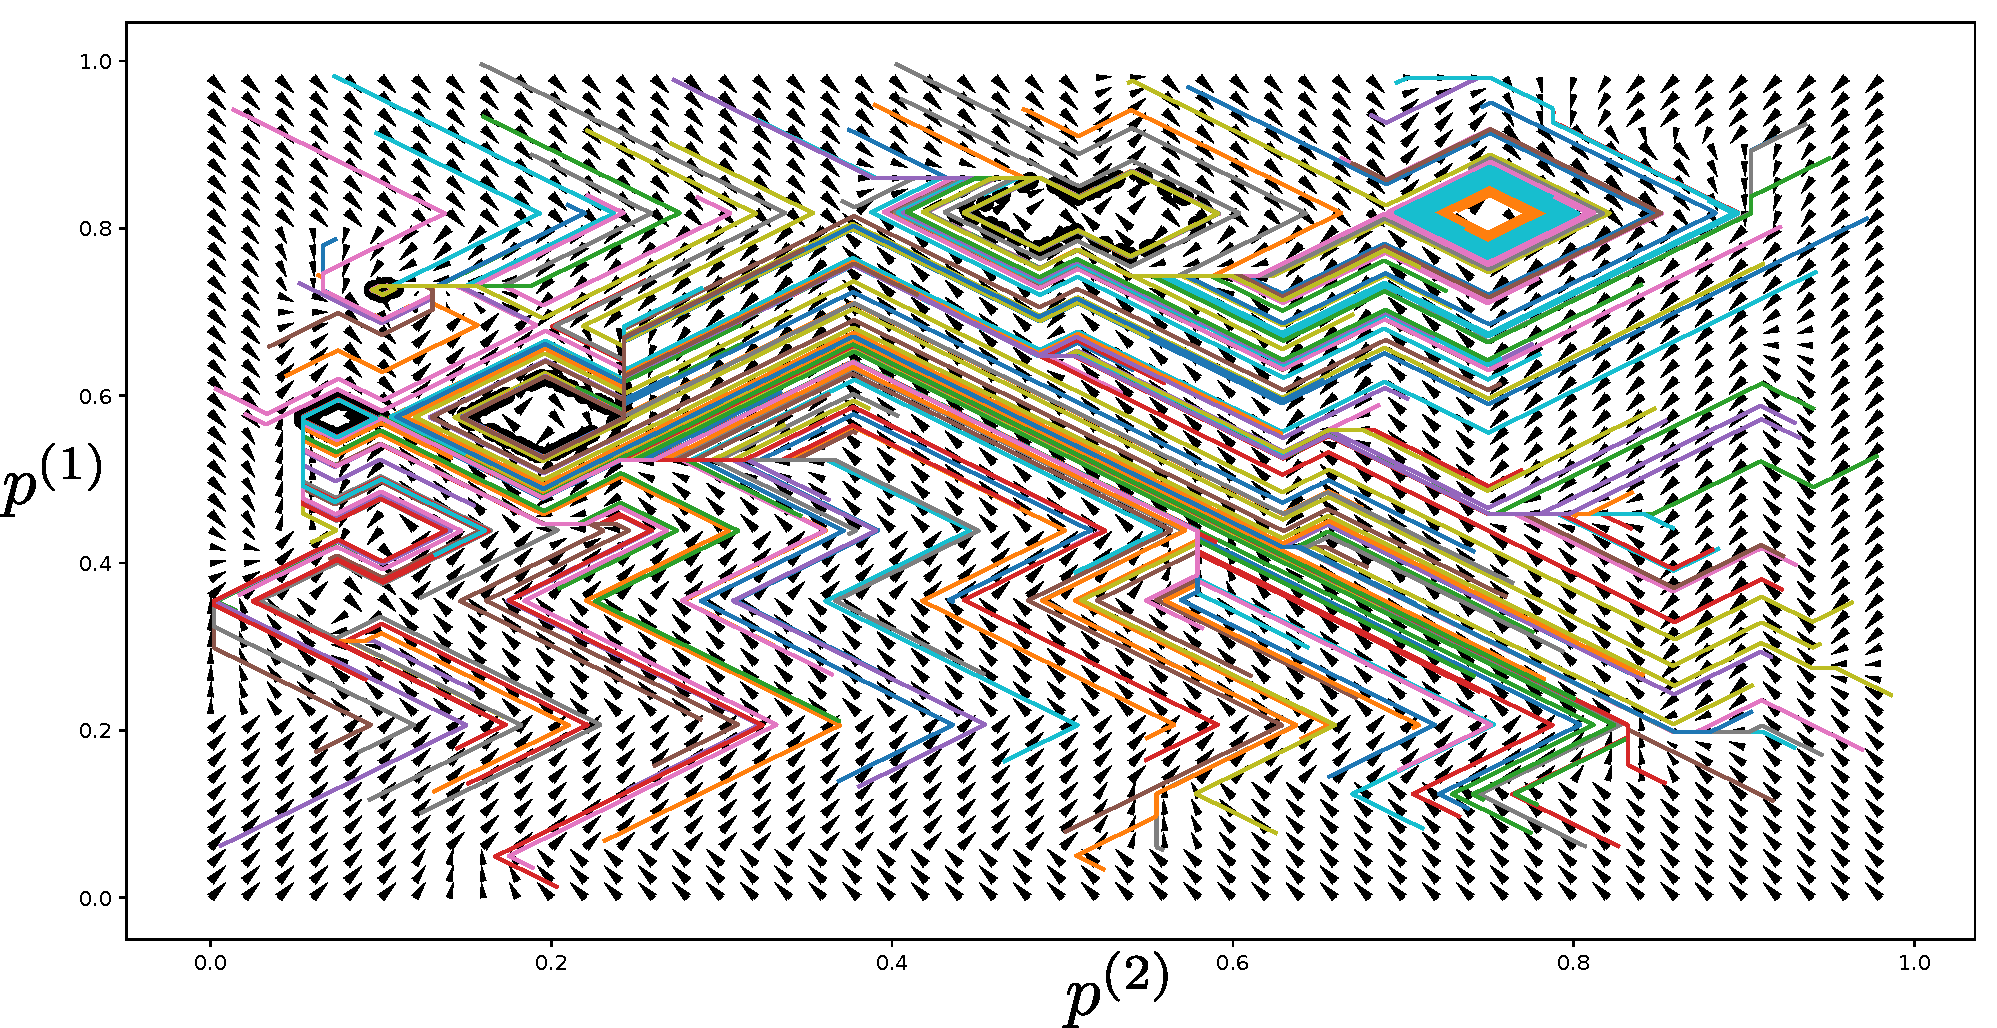
\includegraphics[width=\textwidth]{champ_006_t1.pdf}
\caption{Champ de déplacements de $\bmu\m{1},\bmu\m{2}$ lorsque les poids sont encore aléatoires, à $t=0$. Les trajectoires de 200 relaxations, initialisées différemment, sont représentées. En fonction de la position initiale des BMUs, la relaxation évolue vers un point fixe ou un cycle limite. }
\label{fig:champ_0}
\end{figure}


\begin{figure}
\centering
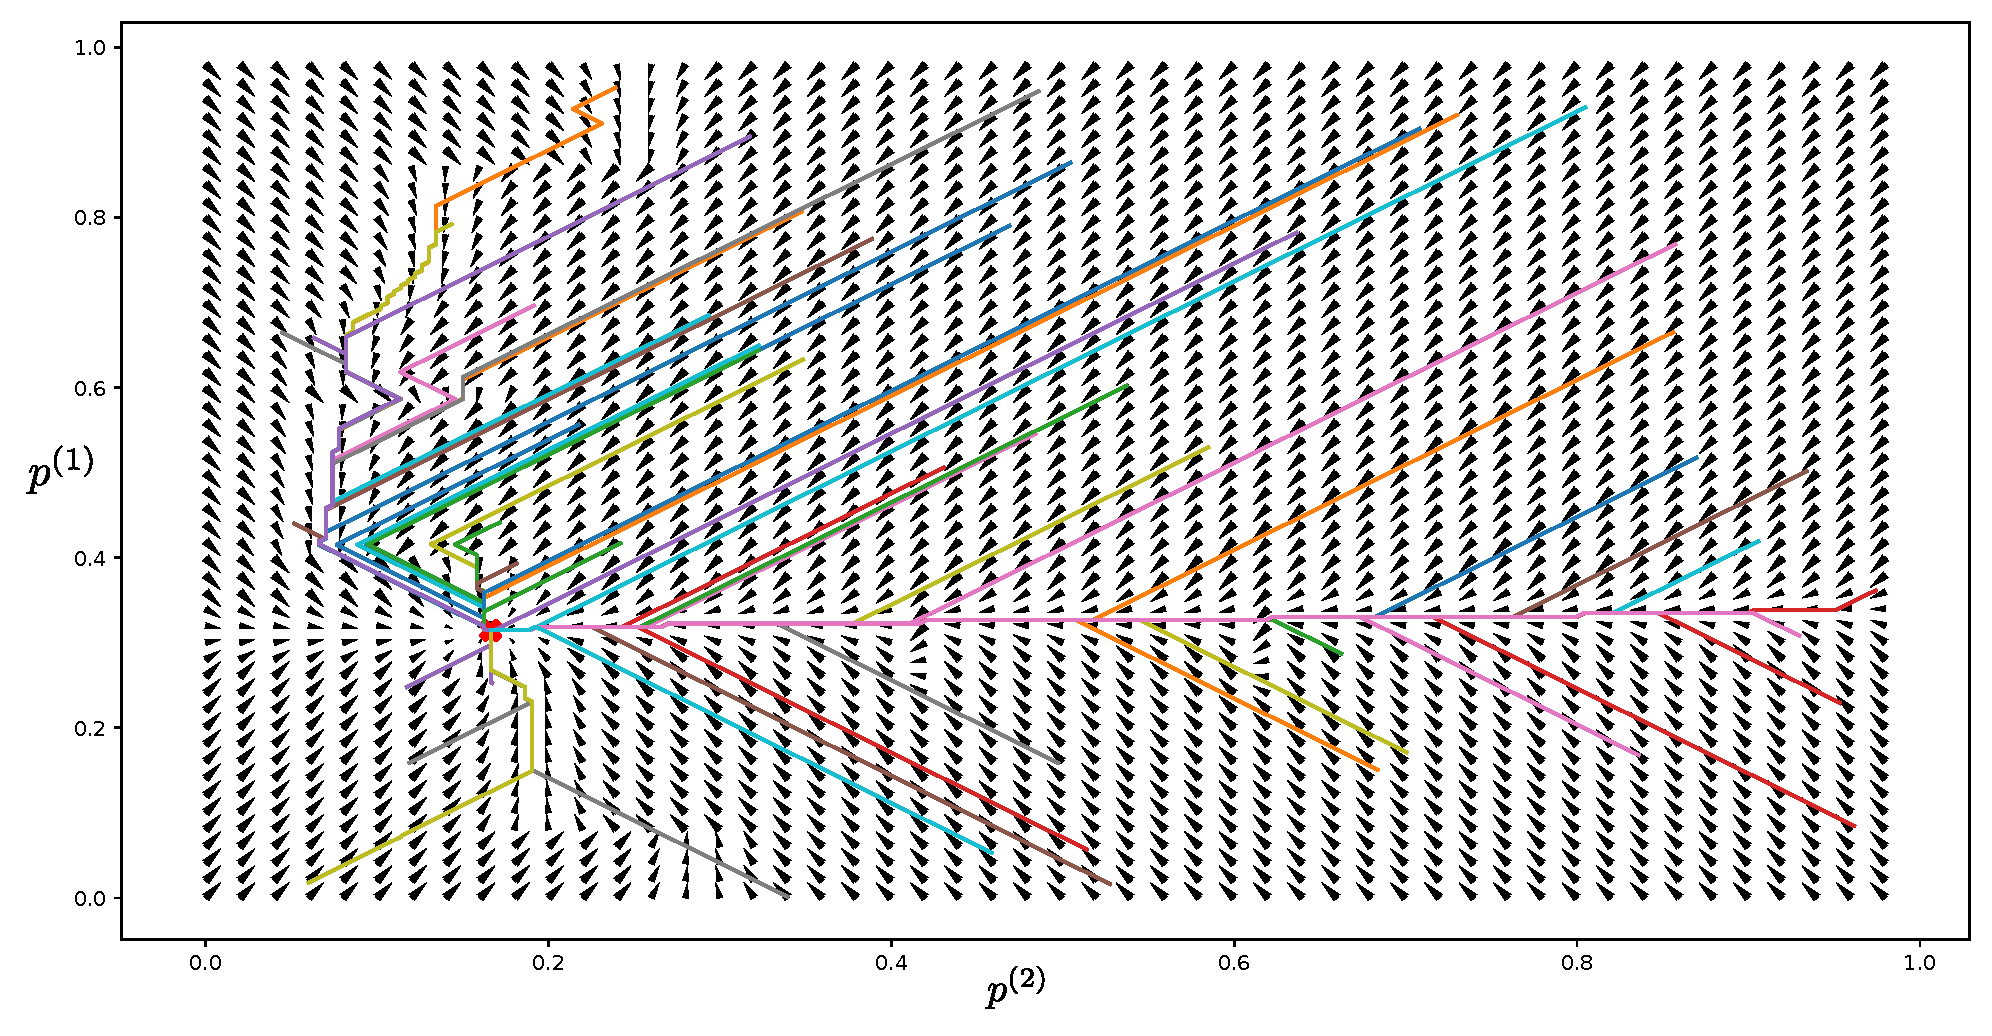
\includegraphics[width=\textwidth]{champ_006.pdf}
\caption{Champ de déplacements de $\bmu\m{1},\bmu\m{2}$ lorsque les poids sont organisés tels que représentés en figure \ref{fig:w006}, à $t=9999$.es trajectoires de 50  relaxations, initialisées différemment, sont représentées. Les relaxations évoluent vers un point fixe commun.}
\label{fig:champ_9999}
\end{figure}

\begin{figure}
	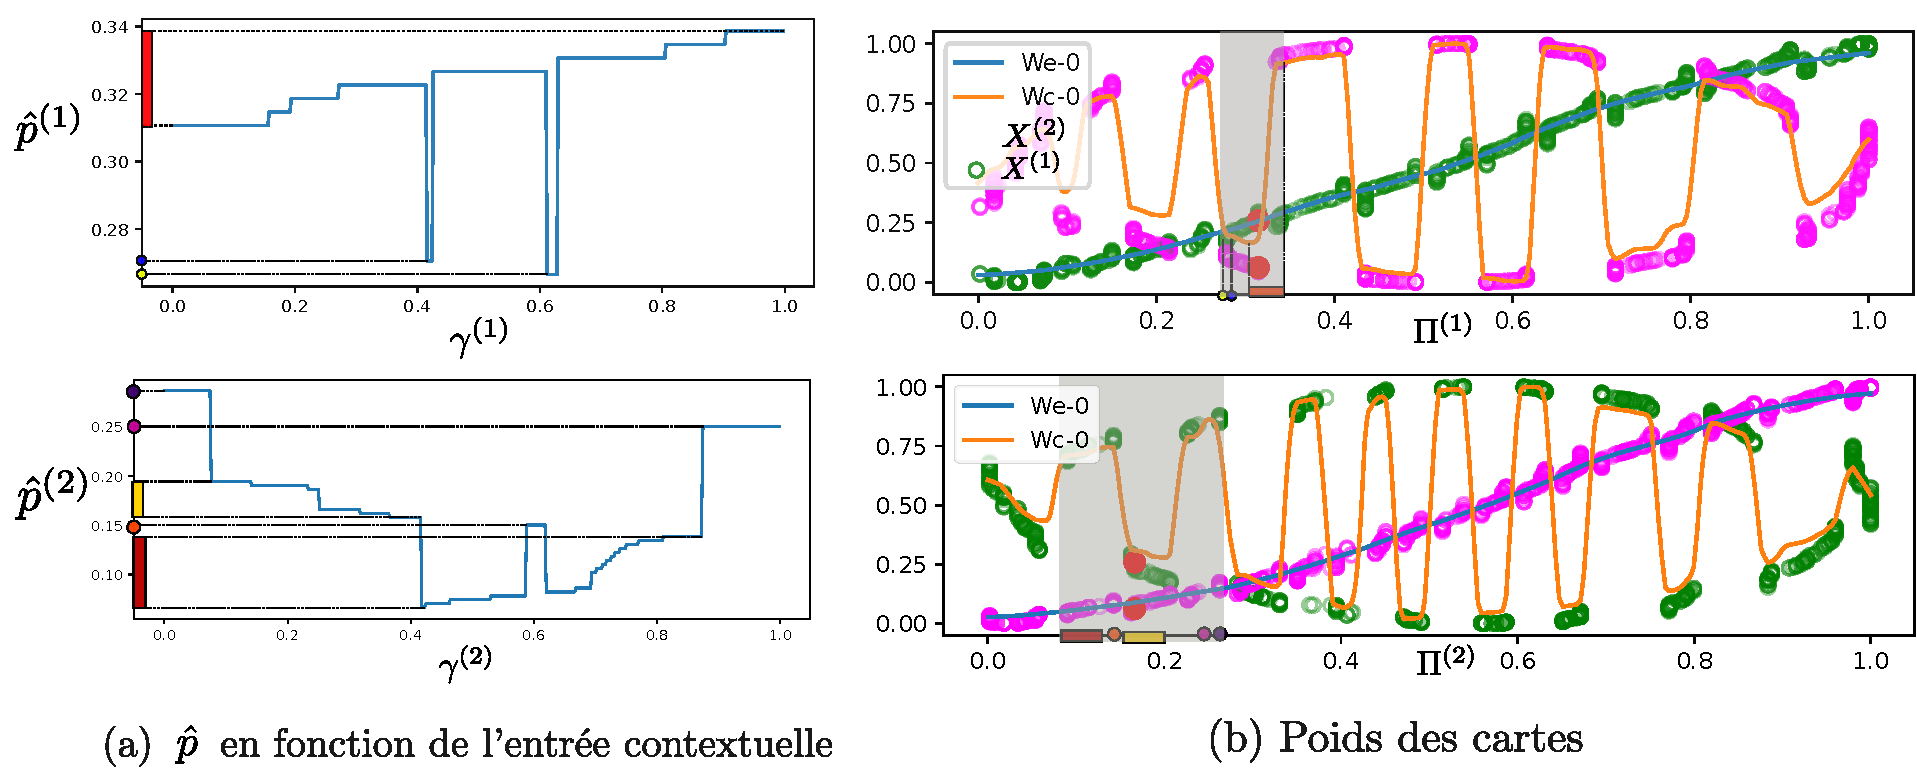
\includegraphics[width=\textwidth]{am_w_006}
	\caption{(a): $\hat{p}\m{1}$ et $\hat{p}\m{2}$ en fonction de l'entrée contextuelle de leur carte $\bmu\m{2}$ et $\bmu\m{1}$.(b): les poids externes et contextuels des cartes $1$ et $2$ sont représentés selon leur position dans la carte. On représente également les entrées test $\inpx\m{1}$ et $\inpx\m{2}$ en fonction de leur BMU. Les entrées utilisées pour tracer les figures de gauche sont colorées en rouge sur les figure de droite: $\inpx\m{1}=0.26,\inpx\m{2}=0.06$. Les intervalles dans lequel les valeurs de $\hat{p}$ varient sont reportés sur la figure (b).}
	\label{fig:w006}
	\end{figure}

\subsection{Influence du pas de relaxation}

Dans les expériences précédentes, nous avons utilisé un pas de convergence $\delta=0.05$.
Une autre solution est de ne pas utiliser de pas de relaxation, c'est à dire, à chaque itération, déplacer le BMU $\bmu\m{i}_\tau$ directement en $\hat{p}\m{i}$, où l'activité globale est maximale, au lieu de le déplacer de $\delta$.
L'évolution de la relaxation devient alors:
\begin{equation}
\forall i, \bmu\m{i}_{\tau+1} = \hat{p}\m{i}_{\tau}
\end{equation}

En figure \ref{fig:diff_nopas}, Nous avons tracé différentes trajectoires de relaxation, pour une même entrée. 
On représente sur cette même figure les différences ${\hat{p}}\m{1} - p\m{1}$ et ${\hat{p}}\m{2} - p\m{2}$. Le point fixé de la fonction génératrice de la suite $(\bmu)_\tau$ est un point pour lequel les deux valeurs sont nulles.
Ces relaxation sont effectués après l'apprentissage des données par l'architecture. La méthode de relaxation utilisée lors de l'apprentissage n'utilise pas non plus de pas de relaxation $\delta$.
A l'issue de l'apprentissage, le comportement de la relaxation ne change pas. 
Cela se comprend au vu des résultats précédents. $\hat{p}\m{1}$ et $\hat{p}\m{2}$ sont dans un intervalle réduit de valeurs de la carte, quelles que soient les positions $p\m{1}$ et $p\m{2}$. Amener directement le BMU dans cet intervalle ou l'y amener pas à pas ne change rien en terme de comportement. 

\begin{figure}
\begin{minipage}{0.5\textwidth}
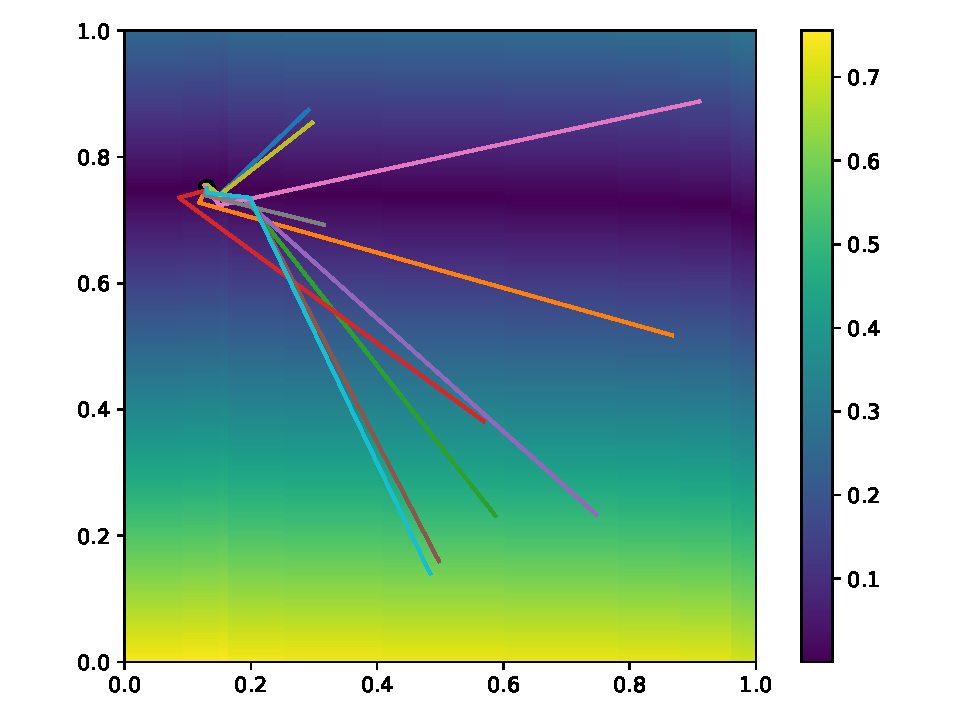
\includegraphics[width=\textwidth]{champ_X_009}
\end{minipage}
\begin{minipage}{0.5\textwidth}
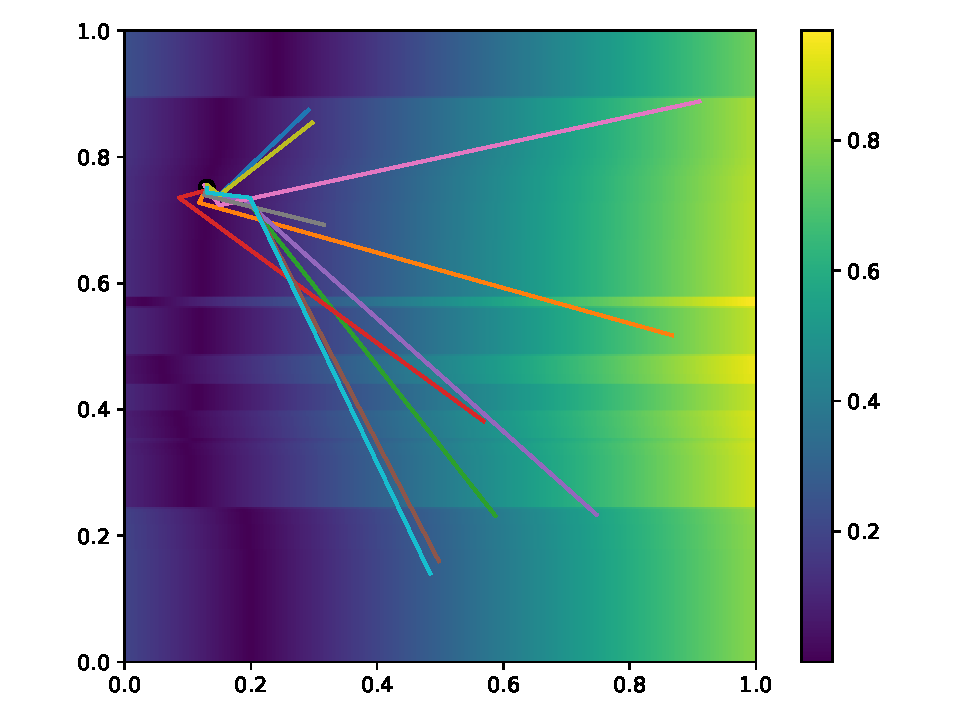
\includegraphics[width=\textwidth]{champ_Y_009}
\end{minipage}
\caption{Trajectoires des relaxations $(\bmu\m{1}_{\tau},\bmu\m{2}_\tau)$ dans le champ des différences ${\hat{p}}\m{1} - p\m{1}$ et ${\hat{p}}\m{2} - p\m{2}$, lorsque la relaxation est effectuée sans utiliser de petits déplacements. Les tracés sont effectués après apprentissage. La relaxation semble encore converger vers un point fixe.}
\label{fig:diff_nopas}
\end{figure}

\section{Conclusion}

Les parties \ref{sec:conv} et \ref{sec:cont} montrent donc que, lorsque les poids sont quelconques, la convergence de l'algorithme de relaxation n'est pas assurée; au contraire, la relaxation évolue dans la plupart des cas vers une situation non convergente. Dans le cas particulier étudié dans la section, il semble exister des point fixes, mais dus au caractère aléatoire des poids. La relaxation ne permet pas de trouver ces points. Pourtant, l'apprentissage des cartes utilisant la relaxation comme recherche de BMU mène une organisation des poids, même sans que la relaxation ne converge au début. Cette organisation permet de plus une meilleure convergence de la relaxation (convergence dans plus de $90 \%$ des cas).

Ce comportement peut être expliqué. On observe que la relaxation converge bien à partir du moment où les poids externes sont organisés et présentent une continuité. 
Au début de l'apprentissage, même si la relaxation mène à des positions quelconques de BMUs, ces BMUs auront quand même des poids externes restant proches de la valeur de l'entrée externe. 
Le calcul de l'activité dépend en effet d'abord de l'activité externe de la carte:
$$ a_g = \sqrt{a_e ( \beta a_e + (1-\beta a_c))}, \;\; \beta=0.5$$ 
De plus, la relaxation est initialisée à une position correspondant au maximum de l'activité externe.

L'organisation de la carte s'effectuera donc de façon similaire à une carte classique. Dans une carte de Kohonen, pour des poids aléatoires, de multiples positions de BMU sont possibles lors du calcul de la distance des poids à l'entrée. La disposition des poids et le choix du BMU n'influencent pas la propriété globale d'organisation d'une carte. Cette même observation peut s'effectuer ici. 
Le rayon de voisinage externe étant bien plus grand que le rayon de voisinage contextuel, l'organisation des poids externes de la carte influence peu l'organisation des poids contextuels.
Lorsque les poids externes présentent une continuité, la relaxation converge. Les poids contextuels peuvent alors s'organiser selon le BMU, qui a maintenant un sens: il s'agit d'un point fixe de la fonction de relaxation. Le BMU correspond alors au point qui maximise en même temps les activités globale de chaque carte.

Expérimentalement, on observe que, lorsque les cartes sont organisés, le point fixe  existe, est unique est est atteint par n'importe quelle trajectoire de relaxation. Le BMU a donc un sens au niveau de la carte. 

Enfin, la relaxation utilise un pas de déplacement utilisé $\delta$. 
On pourrait supposer que prendre un petit $\delta$ permet une meilleure convergence; en fait, la valeur de $\delta$ influence peu la capacité de convergence et l'organisation des cartes. La relaxation pourrait être effectuée sans utiliser de pas de relaxation. Par ailleurs, la relaxation est initialisée proche de la position théorique du BMU, quand elle existe. La relaxation est donc finalement assez courte.

La relaxation est donc une recherche d'un maximum global à l'architecture, ce maximum étant un point fixe de la fonction de mise à jour des positions.
Une fois que les poids externes d'une carte présentent une continuité, la relaxation et le BMU issu de ce processus ont un sens topologique: on observe expérimentalement que la fonction de mise à jour présente un point fixe $\mathbf{\bmu} = \mathbf{f}(\mathbf{\bmu})$, et que la relaxation converge vers ce point fixe. Ce point fixe est alors le point qui maximise \emph{collectivement} les activités globales de chaque carte de l'architecture.
Bien que la relaxation ne converge pas au début de l'apprentissage, la convergence est observée dès que les poids externes présentent une certaine continuité. Cette continuité étant assurée après quelques itérations d'apprentissage par l'algorithme de mise à jours des poids de Kohonen, on peut donc dire que la relaxation converge au sein de CxSOM.
La relaxation est alors un moyen de trouver un ensemble de BMU au sein d'une architecture maximisant une propriété \emph{globale} à cette architecture: toutes les cartes voient leur activité globale maximisée. 
Cette recherche de maximum est réalisée localement, au niveau de chaque carte, et non de façon globale. La relaxation agit alors comme une manière de connecter des cartes de façon non-hiérarchique et les BMUs sont l'interface entre modules de la carte.

\ifSubfilesClassLoaded{
    printbibliography
    %\externaldocument{../main.tex}   
}{}
\end{document}
